The MOSFET inverter circuit is shown below:

\FloatBarrier
\begin{figure}[h!]
	\centering
	\caption{MOSFET Inverter Circuit}
	\label{fig:mos_inverter}
	\begin{circuitikz}
		\draw
		( 0 , 0 ) node[ nmos ] (my_nmos) {$V_{out}$}
		
		% Gate
		(my_nmos.G) to [ short ] ++( -2 , 0 ) coordinate(g_out)
		(g_out) to [ sqV , v<=$V_{in}$ ] ++( 0 , -2 ) coordinate(gnd_1)
		(gnd_1) node[ ground ] (my_gnd_1) {}
		
		% Drain
		(my_nmos.D) to [ R={$300\Omega$} ] ++( 0 , 2 ) coordinate(vcc)
		(vcc) to [ battery , v<=$V_{cc}\rightarrow5V$ ] ++( 2 , 0 ) coordinate(gnd_3)
		(gnd_3) node[ ground ] (my_gnd_3) {}
		
		% Source
		(my_nmos.S) node[ ground ] (my_e_gnd) {}
		
		;
	\end{circuitikz}
\end{figure}

Consider the case when $V_{in}$ is low (close to ground). The MOSFET's gate is set to the ground voltage, the source and the gate are at the same voltage. Typically, the bulk and source are connected to the same node. Thus, if the source is grounded, the bulk is as well. Because the bulk and gate are grounded, the channel does not form because no excess electrons are attracted to the area under the gate. So, the channel cannot conduct carriers to the drain. Thus, no current flows through the MOSFET.

This operation mode is known as the cutoff region. Each MOSFET has what is known as a threshold voltage $V_{Th}$. A MOSFET is said to be in the cutoff region and thus abide by this physical description when the following condition holds:

\begin{equation}
	\label{eq:mos_cutoff}
	V_{GS} \leq V_{Th}
\end{equation}

When the gate voltage does not exceed the source voltage by an amount greater than the threshold voltage $V_{Th}$, the MOSFET cannot conduct a current.

Because no current flows through the MOSFET in the cutoff region, no current flows through the resistor connected to its drain terminal. By Ohm's Law, the voltage drop over the resistor is $0$\si{\volt}. Since the MOSFET and the resistor are in series and the resistor consumes no voltage, the MOSFET must consume a voltage equivalent to the supply voltage $V_{cc}$. Therefore, the output voltage $V_{out}$ is high when the input voltage $V_{in}$ is low.

When $V_{in}$ is high, the gate voltage is higher than the grounded source voltage. Because the gate voltage is high, the gate is now at a higher voltage than the grounded bulk. Thus, excess electrons are attracted from the bulk to the area just beneath the gate oxide. These excess electrons increase the conductivity of this area, producing a conductive channel.

Assume the MOSFET is in saturation mode. A MOSFET is said to be in saturation mode when the following condition holds:

\begin{equation}
	\label{eq:sat_mode}
	V_{GS} - V_{Th} < V_{DS} \rightarrow V_{GD} < V_{Th}
\end{equation}

In saturation mode, current can flow through the MOSFET. However, increasing $V_{G}$ causes the drain current $I_{D}$ to level off. Because $V_{GD} < V_{Th}$, the depletion region between the bulk and the drain limits current flow. When $V_{G}$ is increased, more conduction electrons are attracted to the channel, but they are also impeded with a stronger electric field when entering the drain. Therefore, increasing $V_{G}$ in this state does not increase the drain current $I_D$.

Because electrons can flow through the MOSFET, a current through the MOSFET $I_D$ is produced. Because current can flow through the MOSFET, the resistor can now consume voltage. This means that the MOSFET receives a smaller fraction of the voltage. Thus, the output voltage $V_{out}$ is low when the input voltage is $V_{in}$ is high. Clearly, this circuit demonstrates inverting characteristics, which is why it is called an "inverter".

However, this inverter is not ideal. It takes time for the MOSFET channel to form when the gate voltage is high. When the gate voltage drops back to ground, it takes time for the excess electrons to recombine and diffuse back into the bulk. Thus, a rise time, fall time, and delays can be measured for the output waveform. 

In the experiment, the circuit is configured so that the MOSFET enters the saturation region when the input is high and the cutoff region when the input is low. The input and output waveforms are displayed below, where the yellow waveform is the input and the green waveform is the output.

\FloatBarrier
\begin{figure}[h!]
	\centering
	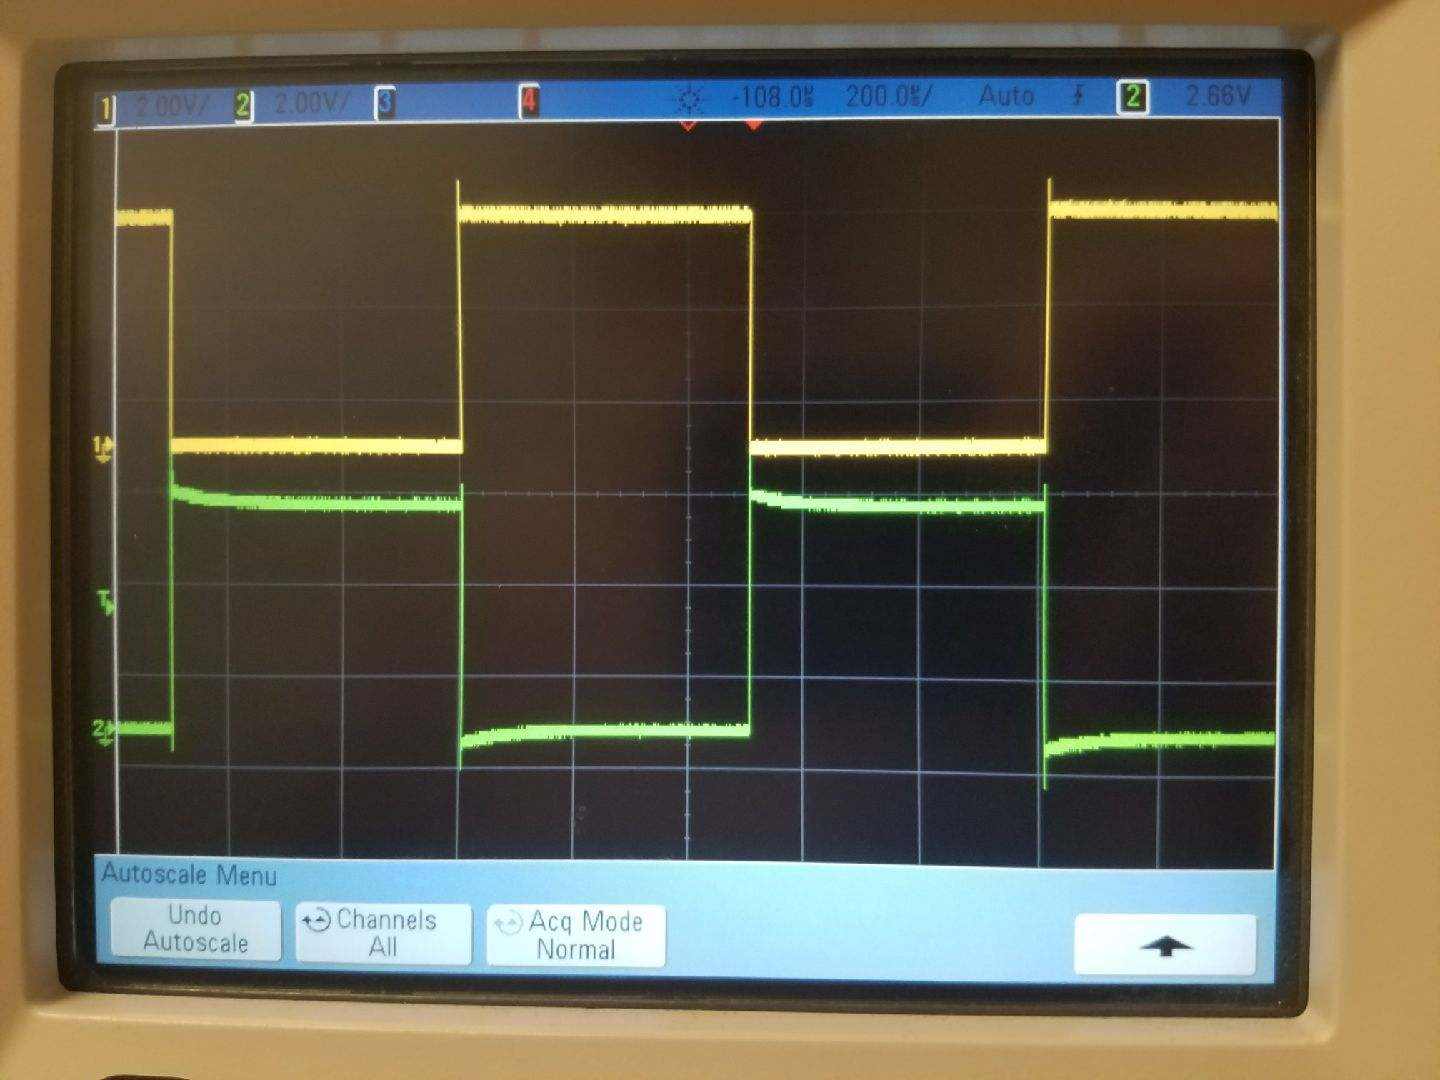
\includegraphics[scale=0.25]{./images/inverter_in_out.jpeg}
	\caption{Inverter Input and Output Voltage}
	\label{fig:inverter_in_out}
\end{figure}
\FloatBarrier

$V_{in}$ is a square pulse with an amplitude of $5$\si{\volt} and a $50\%$ duty cycle. When the input is high, the output is low. Here, $V_{GS}$ is simply $V_{in}$. $V_{DS}$ is $V_{out}$. In experiment 6, the threshold voltage $V_{Th}$ is determined to be about $2$\si{\volt}. So, using equation (\ref{eq:sat_mode}), $V_{GS} - V_{Th} = 5 - 2 = 3 < 5 = V_{DS}$, the transistor is in saturation when the input is high. When the input is low, using equation (\ref{eq:mos_cutoff}), $V_{GS} = 0 < 2 = V_{Th}$. So, the transistor is in the cutoff region when the input is low.

The rise time is measured by acquiring the time it takes for the output voltage to transition from $10\%$ to $90\%$ of its maximum value. It is determined to be about $24$\si{\nano\second}.

\FloatBarrier
\begin{figure}[h!]
	\centering
	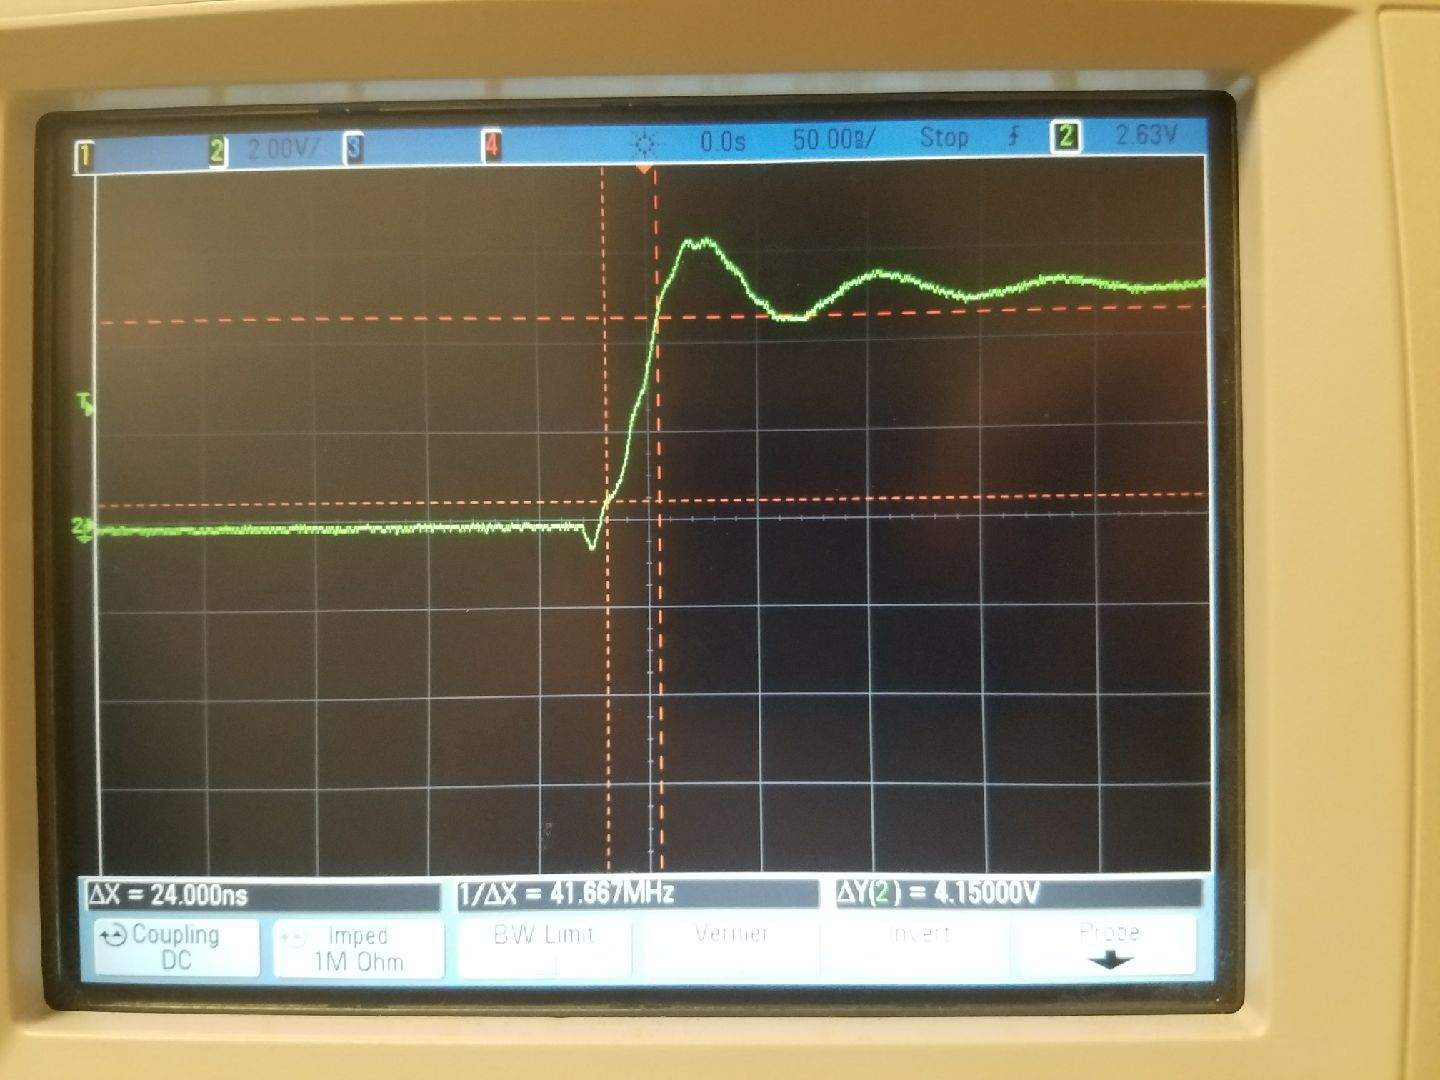
\includegraphics[scale=0.25]{./images/inverter_tr.jpeg}
	\caption{Inverter Rise Time Measurement}
	\label{fig:inverter_rise_time}
\end{figure}
\FloatBarrier

The fall time is found by measuring the time it takes for the output voltage to drop from $90\%$ to $10\%$ of the peak value. It is found to be $14.4$\si{\nano\second}.

\FloatBarrier
\begin{figure}[h!]
	\centering
	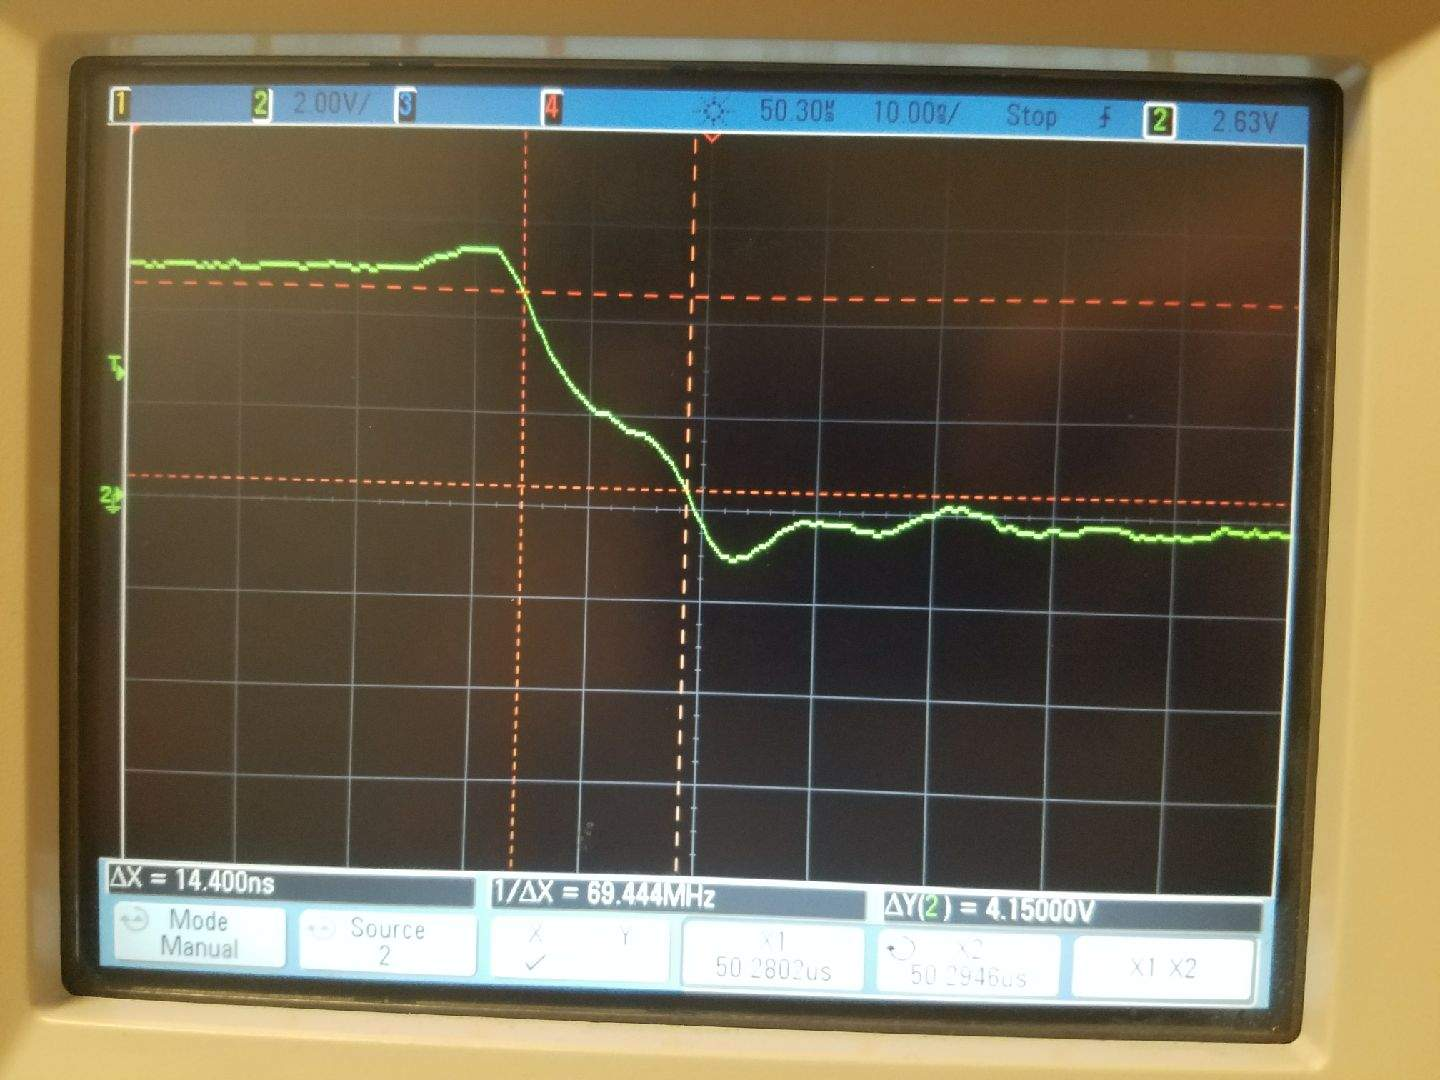
\includegraphics[scale=0.25]{./images/inverter_tf.jpeg}
	\caption{Inverter Fall Time Measurement}
	\label{fig:inverter_fall_time}
\end{figure}
\FloatBarrier

Next, the delay between the input and output when the transistor transitions from cutoff to saturation is measured. This is the same as the delay from the rising edge of the input to the falling edge of the output. The delay is measured from the $50\%$ point on the input to the $50\%$ point on the output.

\FloatBarrier
\begin{figure}[h!]
	\centering
	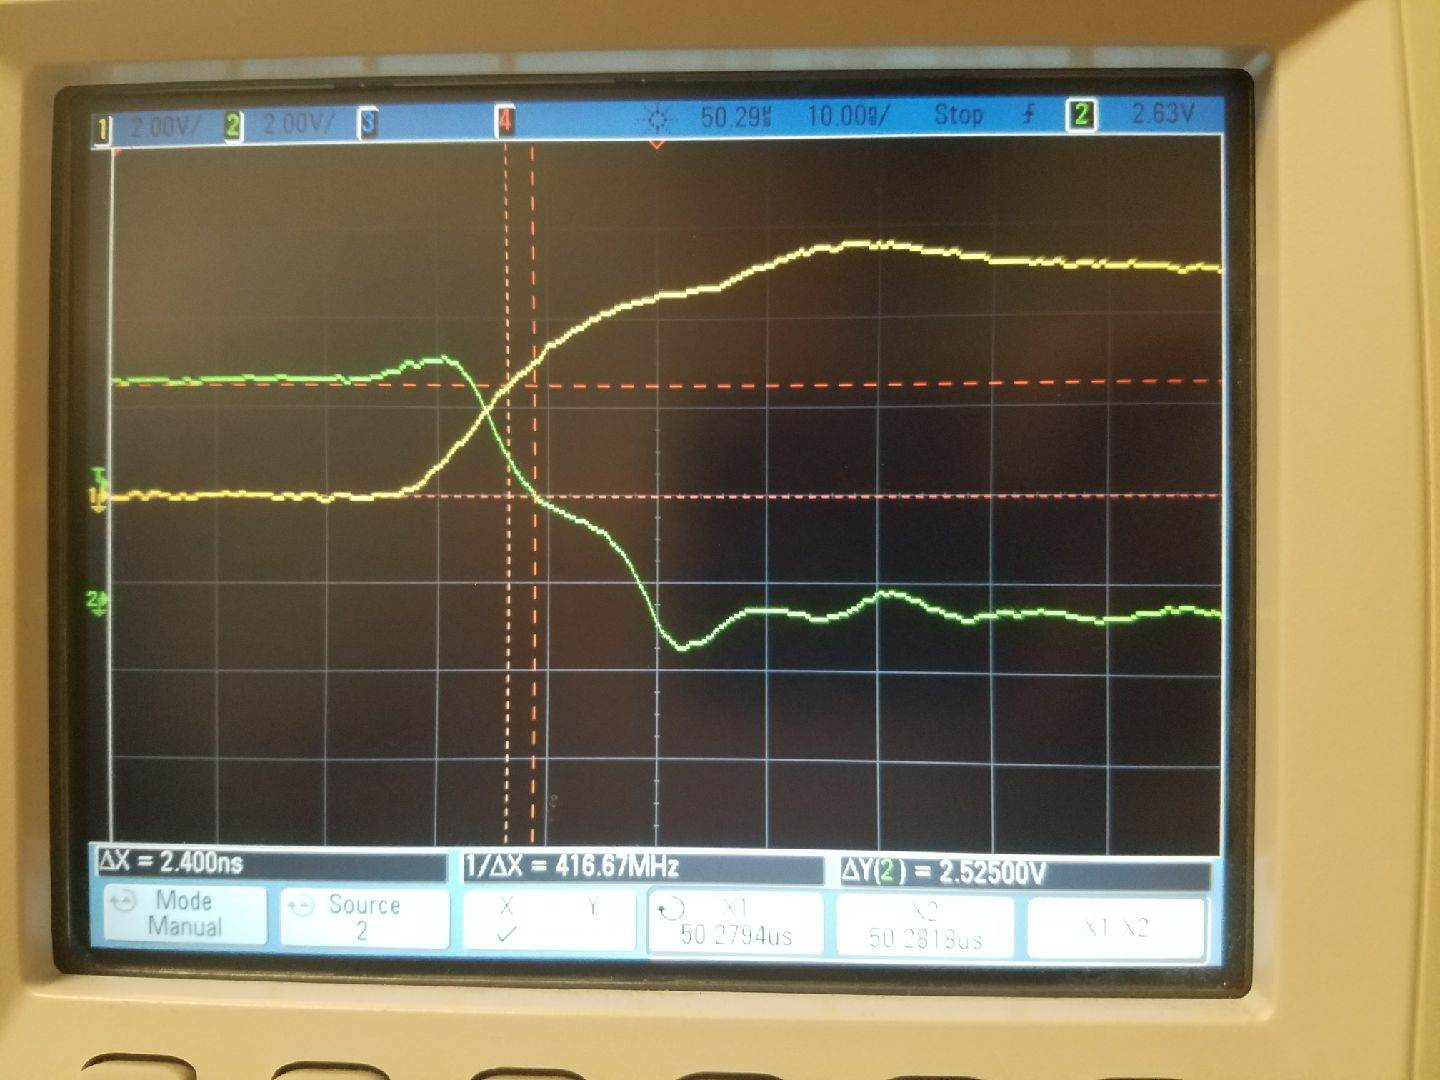
\includegraphics[scale=0.25]{./images/inverter_input_rising_td.jpeg}
	\caption{Inverter Delay Measurement}
	\label{fig:inverter_time_delay}
\end{figure}
\FloatBarrier

This delay is measured to be $2.4$\si{\nano\second}. In the same manner, the delay from saturation to cutoff is measured to be $10.4$\si{\nano\second}.

\FloatBarrier
\begin{table}[h!]
	\centering
	\caption{Inverter Times}
	\label{tab:inverter_times}
	\csvautotabular{./tables/inverter_times.csv}
\end{table}
\FloatBarrier

The delays and rise/fall times limit the MOSFET's frequency performance. At a high frequency, say $3$\si{\giga\hertz}, the period is very short, about $0.33$\si{\nano\second}. When the MOSFET transitions from cutoff to saturation, the response is delayed by $2.4$\si{\nano\second}, more than an order of magnitude longer than a half-period. Thus, at this frequency, the MOSFET could not transition from state to state since it would not have enough time to transition before the input voltage changes back to its original value. This issue is also not limited to switching applications. MOSFET-based amplifiers are also limited in their amplification abilities at high frequencies.
